\documentclass{ximera}
%% handout
%% nohints
%% space
%% newpage
%% numbers

%% You can put user macros here
%% However, you cannot make new environments

\graphicspath{{./}{firstExample/}{secondExample/}}

\usepackage{url}
\usepackage{tikz}
\usepackage{tkz-euclide}
\usetkzobj{all}


\tikzstyle geometryDiagrams=[ultra thick,color=blue!50!black]
\pgfplotsset{compat=1.8}
  \usepackage[T1]{fontenc}
  \usepackage[utf8x]{inputenc}



\title{Optimization}

\begin{document}

\begin{abstract}
We minimize or maximize various quantities.
\end{abstract}
\maketitle

\subsection*{Basic learning objectives}

These are the tasks you should be able to perform with reasonable fluency \textbf{when you arrive at our next class meeting}. Important new vocabulary words are indicated \emph{in italics}. 

\begin{itemize}
	\item Use WolframAlpha or Desmos to solve equations.
    \item Memorize the basic formulas for area and volume.
\end{itemize}

\subsection*{Advanced learning objectives}

In addition to mastering the basic objectives, here are the tasks you should be able to perform \textbf{after class, with practice}: 

\begin{itemize}
	\item Find the formula for an function that we want to minimize or maximize.
    \item Be able to find a maximum or minimum value of a curve.
    \item State the conclusion to the optimization problem as a complete, descriptive sentence.
\end{itemize}

\noindent\hrulefill

We have used many web tools to help us in our computations for this course. In this unit we are using \href{http://wolframalpha.com} and \href{http://desmos.com} to serve as graphing calculators for us. 

In this section we are trying to optimize various functions. When we say the word ``optimize'' we mean that we are trying to find the minimum or maximum output values of the function. For example, we might want to minimize costs or maximize profit.

First we want to show/remind you how useful \href{http://wolframalpha.com} is at solving equations.

\begin{question}
Find the number of solutions to the system of equations:
\[
\begin{cases}
y&=x^3-4x\\
y&=x
\end{cases}
\]

The system has \answer{3} solutions
\begin{hint}
Either plot it in Desmos and count the number of intersection points or just type both equations into WolframAlpha.
\end{hint}

\end{question}



\begin{question}
Find the of solutions to the system of equations:
\[
\begin{cases}
y&=x^3-9x\\
y&=-2x+6
\end{cases}
\]

There are $3$ solutions. 
When $x=-2$, $y=$ \answer{10}
When $x=-1$, $y=$ \answer{8}
When $x=3$, $y=$ \answer{0}

\begin{hint}
Either plot it in Desmos and click on the points where the curves intersect or just type in both equations to WolframAlpha.
\end{hint}

\end{question}

Both Wolfram Alpha and Desmos have the ability to help us find the minimum or maximum value(s) of curves. 

\begin{question}
Find the $y$-coordinate of the highest point on the curve $y=4x^3-x^4$. 

In \href{http://wolframalpha.com} you can  get the answer by entering \verb|maximize 4x^3-x^4|. In \href{http://desmos.com} you can define the curve $y=4x^3-x^4$. Then (with that cell still selected) you can click on the point at the top of the curve to get its coordinates.


The maximum $y$ value is $y=$ \answer{27}.

\end{question}



\begin{question}
In this problem we consider the problem of creating a box by taking a $\SI{6}{in}\times\SI{8}{in}$ sheet and cutting out square corners and folding up the sides as pictured below.
\begin{image}
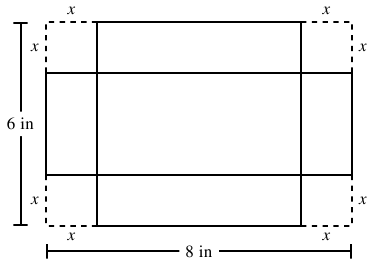
\includegraphics{Optimization1.png}
%\begin{tikzpicture}[line width=1pt]
%\draw (-2,-1) rectangle (2,1) (-2,-2) rectangle (2,2) (-3,-1) rectangle (3,1);
%\draw[style=dashed] (-3,-1) --node[left]{$x$}(-3,-2) --node[below]{$x$} (-2,-2);
%\draw[style=dashed] (3,-1) --node[right]{$x$}(3,-2) --node[below]{$x$} (2,-2);
%\draw[style=dashed] (-3,1) --node[left]{$x$}(-3,2) --node[above]{$x$} (-2,2);
%\draw[style=dashed] (3,1) --node[right]{$x$}(3,2) --node[above]{$x$} (2,2);
%\draw[|-|] (-3.5,-2) --node[fill=white]{$6$ in} (-3.5,2);
%\draw[|-|] (-3,-2.5) --node[fill=white]{$8$ in} (3,-2.5);
%\end{tikzpicture}
\end{image}

We will ignore the units for much of the calculation, but we need to put them back in at the end. The length of the sheet is $8$ so the length of the box (after we have removed the corners) is \answer{8-2x}.
\begin{hint}
When the box is folded it looks like
\begin{image}
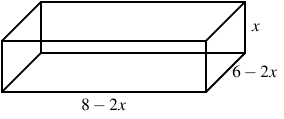
\includegraphics{Optimization2.png}
%\begin{tikzpicture}[line width=1pt,scale=.5]
%\draw (0,0,0) -- (8,0,0) --node[right]{$x$} (8,2,0) -- (0,2,0) -- cycle;
%\draw (0,0,4) --node[below]{$8-2x$} (8,0,4) -- (8,2,4) -- (0,2,4) -- cycle;
%\draw (0,0,0) -- (0,0,4) (8,0,0) --node[right]{$6-2x$}(8,0,4) (8,2,0) -- (8,2,4) (0,2,0) -- (0,2,4);
%\end{tikzpicture}
\end{image}
\end{hint}
The width of the sheet is $6$ so the width of the box is \answer{6-2x}. The height of the box is \answer{x}. 

The volume of the box (in $\si{in^3}$) is given by the formula $V(x)=$ \answer{x(8-2x)(6-2x)}.
\begin{hint}
$\text{Volume}=\text{length}\times\text{width}\times\text{height}$.
\end{hint}

Now go to \href{http://wolframalpha.com} and enter \texttt{maximize x(8-2x)(6-2x)} to find the value of $x$ that maximizes the volume. 

Alternatively, use the function $V(x)=x(8-2x)(6-2x)$ in \href{http://desmos.com} and click the dot at the top of the hump of the curve to see the coordinates of the point at that maximum value.

The side length of each corner square is  $x=$ \answer{1.13} inches.

\end{question}


Memorize the formulas below. We will assume you know them in class and on the test.
\begin{image}
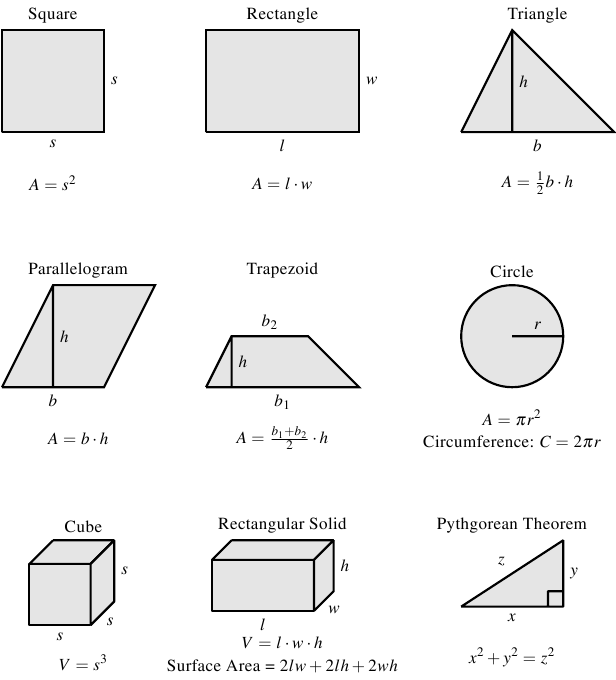
\includegraphics{Optimization3.png}
%\begin{tikzpicture}[line width=1.2pt]
%\begin{scope}
%\draw[fill=gray!20] (0,0) --node[below]{$s$} (2,0) --node[right]{$s$} (2,2) -|(0,0);
%\draw (1,2) node[above]{Square};
%\draw (1,-1) node{$A=s^2$};
%\end{scope}
%
%\begin{scope}[xshift=4cm]
%\draw[fill=gray!20] (0,0) --node[below]{$l$} (3,0) --node[right]{$w$} (3,2) -|(0,0);
%\draw (1.5,2) node[above]{Rectangle};
%\draw (1.5,-1) node{$A=l\cdot w$};
%\end{scope}
%
%\begin{scope}[xshift=9cm]
%\draw[fill=gray!20] (0,0) --node[below]{$b$} (3,0) -- (1,2) --(0,0) (1,0) --node[right]{$h$} (1,2);
%\draw (1.5,2) node[above]{Triangle};
%\draw (1.5,-1) node{$A=\frac{1}{2}b\cdot h$};
%\end{scope}
%
%\begin{scope}[yshift=-5cm]
%\draw[fill=gray!20] (0,0) --node[below]{$b$} (2,0) -- (3,2) -- (1,2) --(0,0) (1,0) --node[right]{$h$} (1,2);
%\draw (1.5,2) node[above]{Parallelogram};
%\draw (1.5,-1) node{$A=b\cdot h$};
%\end{scope}
%
%\begin{scope}[yshift=-5cm,xshift=4cm]
%\draw[fill=gray!20] (0,0) --node[below]{$b_1$} (3,0) -- (2,1) --node[above]{$b_2$} (.5,1) --(0,0) (.5,0) --node[right]{$h$} (.5,1);
%\draw (1.5,2) node[above]{Trapezoid};
%\draw (1.5,-1) node{$A=\frac{b_1+b_2}{2}\cdot h$};
%\end{scope}
%
%\begin{scope}[yshift=-5cm,xshift=9cm]
%\draw[fill=gray!20] (1,1) circle (1cm) (1,1) --node[above]{$r$}++(1,0);
%\draw (1,2) node[above]{Circle};
%\draw (1,-.6) node(A) {$A=\pi r^2$};
%\draw (A) node[below=.2cm]{Circumference: $C=2\pi r$};
%\end{scope}
%
%\begin{scope}[yshift=-9.2cm,xshift=1cm,line join=bevel,scale=1.2]
%\draw[fill=gray!20] (0,1,0) -- (1,1,0) -- (1,1,1) -- (0,1,1) -- (0,1,0);
%\draw[fill=gray!20] (1,0,1) -- node[below]{$s$}(0,0,1)-- (0,1,1) -- (1,1,1) -- (1,0,1);
%\draw[fill=gray!20] (1,1,0) --node[right]{$s$} (1,0,0) --node[below right=-.05cm]{$s$} (1,0,1) -- (1,1,1) -- cycle;
%\draw (.5,1) node[above]{Cube};
%\draw (.5,-1) node{$V=s^3$};
%\end{scope}
%
%\begin{scope}[yshift=-9cm,xshift=4.5cm,line join=bevel]
%\draw[fill=gray!20] (0,1,0) -- (2,1,0) -- (2,1,1) -- (0,1,1) -- (0,1,0);
%\draw[fill=gray!20] (2,0,1) -- node[below]{$l$}(0,0,1)-- (0,1,1) -- (2,1,1) -- (2,0,1);
%\draw[fill=gray!20] (2,1,0) --node[right]{$h$} (2,0,0) --node[below right=-.05cm]{$w$} (2,0,1) -- (2,1,1) -- cycle;
%\draw (1,1) node[above]{Rectangular Solid};
%\draw (1,-1) node (V){$V=l\cdot w\cdot h$};
%\draw (V) node[below=.2cm]{Surface Area = $2lw+2lh+2wh$};
%\end{scope}
%
%\begin{scope}[yshift=-9.3cm,xshift=9cm,line join=bevel]
%\draw[fill=gray!20] (0,0) --node[below]{$x$} (2,0) --node[right]{$y$} (2,1.3) --node[above left]{$z$}(0,0) (2,0) rectangle ++(-.3,.3);
%\draw (1,1.3) node[above]{Pythgorean Theorem};
%\draw (1,-1) node{$x^2+y^2=z^2$};
%\end{scope}
%\end{tikzpicture}
\end{image}





\end{document}
